\section{Ověření modelu}

Pro ověření modelu, je spočítána střední absolutní procentní chyba (MAPE) a koeficient determinace (r2) stejně jako v článku \cite{Hassan}.

\[ MAPE = \frac{100}{n}\displaystyle{\sum_{t=1}^{n} |\frac{A_t-F_t}{A_t}|} \]
kde \(A_t\) je aktuální hodnota a \(F_t\) je předpoveď v čase t.

\clearpage

\section{Výsledky}

\subsection{Testovací scénář}

Pro otestování modelu byl použit index S\&P 500 jako v případě \cite{Nguyen} (ticker SPY), ale byly použity historické denní
ceny od 1.1.2019 do 1.1.2022 na časové okno 100 dní, tedy na 2.1.2022 a 100 (obchodních) dní zpět.
\begin{lstlisting}
python -m hmm_stock_forecast.main -s 2019-01-01 -e
2022-01-01 -t SPY -w 100
\end{lstlisting}

\subsection{Optimální počet stavů}
Program našel optimální počet stavů dle zmíněných kritérií na 2 stavy a vykreslil grafy pro jednotlivá kritéria
viz obrázek \ref{fig:aic} pro AIC.

\begin{figure}[h]
    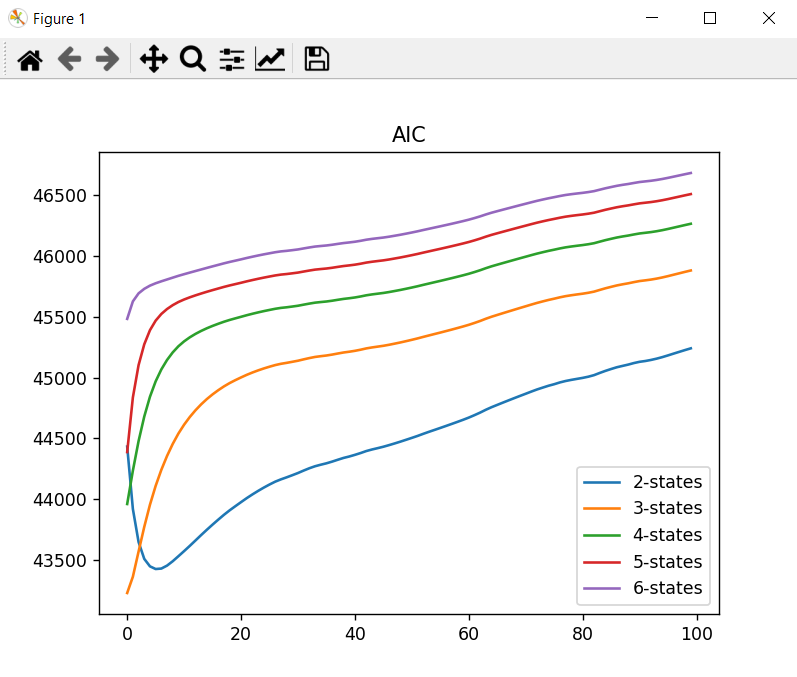
\includegraphics[width=1\textwidth]{img/aic}
    \caption{AIC}
    \label{fig:aic}
\end{figure}

\subsection{Predikce cen}
Na obrázku \ref{fig:result} je vidět graf predikovaných a reálných cen na časové okno 2.1.2022 a 100 (obchodních) dní zpět.

\begin{figure}[h]
    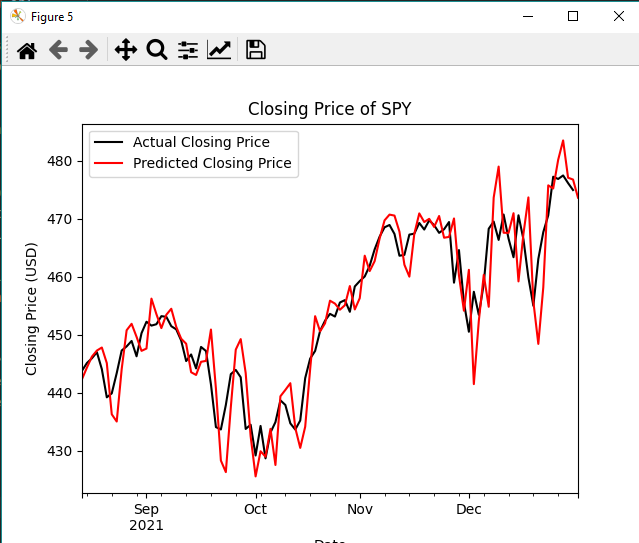
\includegraphics[width=1\textwidth]{img/result}
    \caption{Výsledek}
    \label{fig:result}
\end{figure}

\subsection{Chyby}
Pro náš testovací scénář vyšly chyb takto:
\[MAPE = 0.861\]
\[r2 = 0.822\]

\subsection{Porovnání s pomegranate}
Stejný test byl proveden také s modelem z knihovny \textbf{pomegranate}, který vybral také jako optimální dva stavy a
výsledek predikce je vidět na obrázku \ref{fig:pomegranate}.
\begin{lstlisting}
python -m hmm_stock_forecast.main -s 2019-01-01 -e
2022-01-01 -t SPY -w 100 -m pomegranate
\end{lstlisting}

\begin{figure}[h]
    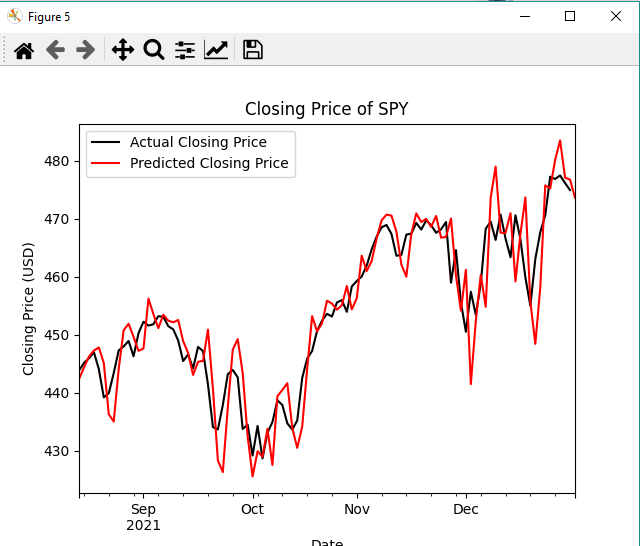
\includegraphics[width=1\textwidth]{img/pomegranate}
    \caption{Výsledek}
    \label{fig:pomegranate}
\end{figure}

\[MAPE = 0.860\]
\[r2 = 0.822\]

Je také nutno podotknout, že model z knihovny \textbf{pomegranate} běží mnohem rychleji z důvodu, že části jsou psané v cythonu a využívá
paralelizace.

\clearpage
